% Created 2022-05-09 Mon 09:57
% Intended LaTeX compiler: pdflatex
\documentclass[11pt]{article}
\usepackage[utf8]{inputenc}
\usepackage[T1]{fontenc}
\usepackage{graphicx}
\usepackage{longtable}
\usepackage{wrapfig}
\usepackage{rotating}
\usepackage[normalem]{ulem}
\usepackage{amsmath}
\usepackage{amssymb}
\usepackage{capt-of}
\usepackage{hyperref}
\graphicspath{{../../books/}}
% wrong resolution of image
% https://tex.stackexchange.com/questions/21627/image-from-includegraphics-showing-in-wrong-image-size?rq=1

%%%%%%%%%%%%%%%%%%%%%%%%%%%%%%%%%%%%%%
%% TIPS                                 %%
%%%%%%%%%%%%%%%%%%%%%%%%%%%%%%%%%%%%%%
% \substack{a\\b} for multiple lines text
% \usepackage{expl3}
% \expandafter\def\csname ver@l3regex.sty\endcsname{}
% \usepackage{pkgloader}
\usepackage[utf8]{inputenc}

% nfss error
% \usepackage[B1,T1]{fontenc}
\usepackage{fontspec}

% \usepackage[Emoticons]{ucharclasses}
\newfontfamily\DejaSans{DejaVu Sans}
% \setDefaultTransitions{\DejaSans}{}

% pdfplots will load xolor automatically without option
\usepackage[dvipsnames]{xcolor}

%                                                             ┳┳┓   ┓
%                                                             ┃┃┃┏┓╋┣┓
%                                                             ┛ ┗┗┻┗┛┗
% \usepackage{amsmath} mathtools loads the amsmath
\usepackage{amsmath}
\usepackage{mathtools}

\usepackage{amsthm}
\usepackage{amsbsy}

%\usepackage{commath}

\usepackage{amssymb}

\usepackage{mathrsfs}
%\usepackage{mathabx}
\usepackage{stmaryrd}
\usepackage{empheq}

\usepackage{scalerel}
\usepackage{stackengine}
\usepackage{stackrel}



\usepackage{nicematrix}
\usepackage{tensor}
\usepackage{blkarray}
\usepackage{siunitx}
\usepackage[f]{esvect}

% centering \not on a letter
\usepackage{slashed}
\usepackage[makeroom]{cancel}

%\usepackage{merriweather}
\usepackage{unicode-math}
\setmainfont{TeX Gyre Pagella}
% \setmathfont{STIX}
%\setmathfont{texgyrepagella-math.otf}
%\setmathfont{Libertinus Math}
\setmathfont{Latin Modern Math}

 % \setmathfont[range={\smwhtdiamond,\enclosediamond,\varlrtriangle}]{Latin Modern Math}
\setmathfont[range={\rightrightarrows,\twoheadrightarrow,\leftrightsquigarrow,\triangledown,\vartriangle,\precneq,\succneq,\prec,\succ,\preceq,\succeq,\tieconcat}]{XITS Math}
 \setmathfont[range={\int,\setminus}]{Libertinus Math}
 % \setmathfont[range={\mathalpha}]{TeX Gyre Pagella Math}
%\setmathfont[range={\mitA,\mitB,\mitC,\mitD,\mitE,\mitF,\mitG,\mitH,\mitI,\mitJ,\mitK,\mitL,\mitM,\mitN,\mitO,\mitP,\mitQ,\mitR,\mitS,\mitT,\mitU,\mitV,\mitW,\mitX,\mitY,\mitZ,\mita,\mitb,\mitc,\mitd,\mite,\mitf,\mitg,\miti,\mitj,\mitk,\mitl,\mitm,\mitn,\mito,\mitp,\mitq,\mitr,\mits,\mitt,\mitu,\mitv,\mitw,\mitx,\mity,\mitz}]{TeX Gyre Pagella Math}
% unicode is not good at this!
%\let\nmodels\nvDash

 \usepackage{wasysym}

 % for wide hat
 \DeclareSymbolFont{yhlargesymbols}{OMX}{yhex}{m}{n} \DeclareMathAccent{\what}{\mathord}{yhlargesymbols}{"62}

%                                                               ┏┳┓•┓
%                                                                ┃ ┓┃┏┓
%                                                                ┻ ┗┛┗┗

\usepackage{pgfplots}
\pgfplotsset{compat=1.18}
\usepackage{tikz}
\usepackage{tikz-cd}
\tikzcdset{scale cd/.style={every label/.append style={scale=#1},
    cells={nodes={scale=#1}}}}
% TODO: discard qtree and use forest
% \usepackage{tikz-qtree}
\usepackage{forest}

\usetikzlibrary{arrows,positioning,calc,fadings,decorations,matrix,decorations,shapes.misc}
%setting from geogebra
\definecolor{ccqqqq}{rgb}{0.8,0,0}

%                                                          ┳┳┓•    ┓┓
%                                                          ┃┃┃┓┏┏┏┓┃┃┏┓┏┓┏┓┏┓┓┏┏
%                                                          ┛ ┗┗┛┗┗ ┗┗┗┻┛┗┗ ┗┛┗┻┛
%\usepackage{twemojis}
\usepackage[most]{tcolorbox}
\usepackage{threeparttable}
\usepackage{tabularx}

\usepackage{enumitem}
\usepackage[indLines=false]{algpseudocodex}
\usepackage[]{algorithm2e}
% \SetKwComment{Comment}{/* }{ */}
% \algrenewcommand\algorithmicrequire{\textbf{Input:}}
% \algrenewcommand\algorithmicensure{\textbf{Output:}}
% wrong with preview
\usepackage{subcaption}
\usepackage{caption}
% {\aunclfamily\Huge}
\usepackage{auncial}

\usepackage{float}

\usepackage{fancyhdr}

\usepackage{ifthen}
\usepackage{xargs}

\definecolor{mintedbg}{rgb}{0.99,0.99,0.99}
\usepackage[cachedir=\detokenize{~/miscellaneous/trash}]{minted}
\setminted{breaklines,
  mathescape,
  bgcolor=mintedbg,
  fontsize=\footnotesize,
  frame=single,
  linenos}
\usemintedstyle{xcode}
\usepackage{tcolorbox}
\usepackage{etoolbox}



\usepackage{imakeidx}
\usepackage{hyperref}
\usepackage{soul}
\usepackage{framed}

% don't use this for preview
%\usepackage[margin=1.5in]{geometry}
% \usepackage{geometry}
% \geometry{legalpaper, landscape, margin=1in}
\usepackage[font=itshape]{quoting}

%\LoadPackagesNow
%\usepackage[xetex]{preview}
%%%%%%%%%%%%%%%%%%%%%%%%%%%%%%%%%%%%%%%
%% USEPACKAGES end                       %%
%%%%%%%%%%%%%%%%%%%%%%%%%%%%%%%%%%%%%%%

%%%%%%%%%%%%%%%%%%%%%%%%%%%%%%%%%%%%%%%
%% Algorithm environment
%%%%%%%%%%%%%%%%%%%%%%%%%%%%%%%%%%%%%%%
\SetKwIF{Recv}{}{}{upon receiving}{do}{}{}{}
\SetKwBlock{Init}{initially do}{}
\SetKwProg{Function}{Function}{:}{}

% https://github.com/chrmatt/algpseudocodex/issues/3
\algnewcommand\algorithmicswitch{\textbf{switch}}%
\algnewcommand\algorithmiccase{\textbf{case}}
\algnewcommand\algorithmicof{\textbf{of}}
\algnewcommand\algorithmicotherwise{\texttt{otherwise} $\Rightarrow$}

\makeatletter
\algdef{SE}[SWITCH]{Switch}{EndSwitch}[1]{\algpx@startIndent\algpx@startCodeCommand\algorithmicswitch\ #1\ \algorithmicdo}{\algpx@endIndent\algpx@startCodeCommand\algorithmicend\ \algorithmicswitch}%
\algdef{SE}[CASE]{Case}{EndCase}[1]{\algpx@startIndent\algpx@startCodeCommand\algorithmiccase\ #1}{\algpx@endIndent\algpx@startCodeCommand\algorithmicend\ \algorithmiccase}%
\algdef{SE}[CASEOF]{CaseOf}{EndCaseOf}[1]{\algpx@startIndent\algpx@startCodeCommand\algorithmiccase\ #1 \algorithmicof}{\algpx@endIndent\algpx@startCodeCommand\algorithmicend\ \algorithmiccase}
\algdef{SE}[OTHERWISE]{Otherwise}{EndOtherwise}[0]{\algpx@startIndent\algpx@startCodeCommand\algorithmicotherwise}{\algpx@endIndent\algpx@startCodeCommand\algorithmicend\ \algorithmicotherwise}
\ifbool{algpx@noEnd}{%
  \algtext*{EndSwitch}%
  \algtext*{EndCase}%
  \algtext*{EndCaseOf}
  \algtext*{EndOtherwise}
  %
  % end indent line after (not before), to get correct y position for multiline text in last command
  \apptocmd{\EndSwitch}{\algpx@endIndent}{}{}%
  \apptocmd{\EndCase}{\algpx@endIndent}{}{}%
  \apptocmd{\EndCaseOf}{\algpx@endIndent}{}{}
  \apptocmd{\EndOtherwise}{\algpx@endIndent}{}{}
}{}%

\pretocmd{\Switch}{\algpx@endCodeCommand}{}{}
\pretocmd{\Case}{\algpx@endCodeCommand}{}{}
\pretocmd{\CaseOf}{\algpx@endCodeCommand}{}{}
\pretocmd{\Otherwise}{\algpx@endCodeCommand}{}{}

% for end commands that may not be printed, tell endCodeCommand whether we are using noEnd
\ifbool{algpx@noEnd}{%
  \pretocmd{\EndSwitch}{\algpx@endCodeCommand[1]}{}{}%
  \pretocmd{\EndCase}{\algpx@endCodeCommand[1]}{}{}
  \pretocmd{\EndCaseOf}{\algpx@endCodeCommand[1]}{}{}%
  \pretocmd{\EndOtherwise}{\algpx@endCodeCommand[1]}{}{}
}{%
  \pretocmd{\EndSwitch}{\algpx@endCodeCommand[0]}{}{}%
  \pretocmd{\EndCase}{\algpx@endCodeCommand[0]}{}{}%
  \pretocmd{\EndCaseOf}{\algpx@endCodeCommand[0]}{}{}
  \pretocmd{\EndOtherwise}{\algpx@endCodeCommand[0]}{}{}
}%
\makeatother
% % For algpseudocode
% \algnewcommand\algorithmicswitch{\textbf{switch}}
% \algnewcommand\algorithmiccase{\textbf{case}}
% \algnewcommand\algorithmiccaseof{\textbf{case}}
% \algnewcommand\algorithmicof{\textbf{of}}
% % New "environments"
% \algdef{SE}[SWITCH]{Switch}{EndSwitch}[1]{\algorithmicswitch\ #1\ \algorithmicdo}{\algorithmicend\ \algorithmicswitch}%
% \algdef{SE}[CASE]{Case}{EndCase}[1]{\algorithmiccase\ #1}{\algorithmicend\ \algorithmiccase}%
% \algtext*{EndSwitch}%
% \algtext*{EndCase}
% \algdef{SE}[CASEOF]{CaseOf}{EndCaseOf}[1]{\algorithmiccaseof\ #1 \algorithmicof}{\algorithmicend\ \algorithmiccaseof}
% \algtext*{EndCaseOf}



%\pdfcompresslevel0

% quoting from
% https://tex.stackexchange.com/questions/391726/the-quotation-environment
\NewDocumentCommand{\bywhom}{m}{% the Bourbaki trick
  {\nobreak\hfill\penalty50\hskip1em\null\nobreak
   \hfill\mbox{\normalfont(#1)}%
   \parfillskip=0pt \finalhyphendemerits=0 \par}%
}

\NewDocumentEnvironment{pquotation}{m}
  {\begin{quoting}[
     indentfirst=true,
     leftmargin=\parindent,
     rightmargin=\parindent]\itshape}
  {\bywhom{#1}\end{quoting}}

\indexsetup{othercode=\small}
\makeindex[columns=2,options={-s /media/wu/file/stuuudy/notes/index_style.ist},intoc]
\makeatletter
\def\@idxitem{\par\hangindent 0pt}
\makeatother


% \newcounter{dummy} \numberwithin{dummy}{section}
\newtheorem{dummy}{dummy}[section]
\theoremstyle{definition}
\newtheorem{definition}[dummy]{Definition}
\theoremstyle{plain}
\newtheorem{corollary}[dummy]{Corollary}
\newtheorem{lemma}[dummy]{Lemma}
\newtheorem{proposition}[dummy]{Proposition}
\newtheorem{theorem}[dummy]{Theorem}
\newtheorem{notation}[dummy]{Notation}
\newtheorem{conjecture}[dummy]{Conjecture}
\newtheorem{fact}[dummy]{Fact}
\newtheorem{warning}[dummy]{Warning}
\theoremstyle{definition}
\newtheorem{examplle}{Example}[section]
\theoremstyle{remark}
\newtheorem*{remark}{Remark}
\newtheorem{exercise}{Exercise}[subsection]
\newtheorem{problem}{Problem}[subsection]
\newtheorem{observation}{Observation}[section]
\newenvironment{claim}[1]{\par\noindent\textbf{Claim:}\space#1}{}

\makeatletter
\DeclareFontFamily{U}{tipa}{}
\DeclareFontShape{U}{tipa}{m}{n}{<->tipa10}{}
\newcommand{\arc@char}{{\usefont{U}{tipa}{m}{n}\symbol{62}}}%

\newcommand{\arc}[1]{\mathpalette\arc@arc{#1}}

\newcommand{\arc@arc}[2]{%
  \sbox0{$\m@th#1#2$}%
  \vbox{
    \hbox{\resizebox{\wd0}{\height}{\arc@char}}
    \nointerlineskip
    \box0
  }%
}
\makeatother

\setcounter{MaxMatrixCols}{20}
%%%%%%% ABS
\DeclarePairedDelimiter\abss{\lvert}{\rvert}%
\DeclarePairedDelimiter\normm{\lVert}{\rVert}%

% Swap the definition of \abs* and \norm*, so that \abs
% and \norm resizes the size of the brackets, and the
% starred version does not.
\makeatletter
\let\oldabs\abss
%\def\abs{\@ifstar{\oldabs}{\oldabs*}}
\newcommand{\abs}{\@ifstar{\oldabs}{\oldabs*}}
\newcommand{\norm}[1]{\left\lVert#1\right\rVert}
%\let\oldnorm\normm
%\def\norm{\@ifstar{\oldnorm}{\oldnorm*}}
%\renewcommand{norm}{\@ifstar{\oldnorm}{\oldnorm*}}
\makeatother

% \stackMath
% \newcommand\what[1]{%
% \savestack{\tmpbox}{\stretchto{%
%   \scaleto{%
%     \scalerel*[\widthof{\ensuremath{#1}}]{\kern-.6pt\bigwedge\kern-.6pt}%
%     {\rule[-\textheight/2]{1ex}{\textheight}}%WIDTH-LIMITED BIG WEDGE
%   }{\textheight}%
% }{0.5ex}}%
% \stackon[1pt]{#1}{\tmpbox}%
% }

% \newcommand\what[1]{\ThisStyle{%
%     \setbox0=\hbox{$\SavedStyle#1$}%
%     \stackengine{-1.0\ht0+.5pt}{$\SavedStyle#1$}{%
%       \stretchto{\scaleto{\SavedStyle\mkern.15mu\char'136}{2.6\wd0}}{1.4\ht0}%
%     }{O}{c}{F}{T}{S}%
%   }
% }

% \newcommand\wtilde[1]{\ThisStyle{%
%     \setbox0=\hbox{$\SavedStyle#1$}%
%     \stackengine{-.1\LMpt}{$\SavedStyle#1$}{%
%       \stretchto{\scaleto{\SavedStyle\mkern.2mu\AC}{.5150\wd0}}{.6\ht0}%
%     }{O}{c}{F}{T}{S}%
%   }
% }

% \newcommand\wbar[1]{\ThisStyle{%
%     \setbox0=\hbox{$\SavedStyle#1$}%
%     \stackengine{.5pt+\LMpt}{$\SavedStyle#1$}{%
%       \rule{\wd0}{\dimexpr.3\LMpt+.3pt}%
%     }{O}{c}{F}{T}{S}%
%   }
% }

\newcommand{\bl}[1] {\boldsymbol{#1}}
\newcommand{\Wt}[1] {\stackrel{\sim}{\smash{#1}\rule{0pt}{1.1ex}}}
\newcommand{\wt}[1] {\widetilde{#1}}
\newcommand{\tf}[1] {\textbf{#1}}

\newcommand{\wu}[1]{{\color{red} #1}}

%For boxed texts in align, use Aboxed{}
%otherwise use boxed{}

\DeclareMathSymbol{\widehatsym}{\mathord}{largesymbols}{"62}
\newcommand\lowerwidehatsym{%
  \text{\smash{\raisebox{-1.3ex}{%
    $\widehatsym$}}}}
\newcommand\fixwidehat[1]{%
  \mathchoice
    {\accentset{\displaystyle\lowerwidehatsym}{#1}}
    {\accentset{\textstyle\lowerwidehatsym}{#1}}
    {\accentset{\scriptstyle\lowerwidehatsym}{#1}}
    {\accentset{\scriptscriptstyle\lowerwidehatsym}{#1}}
  }


\newcommand{\cupdot}{\mathbin{\dot{\cup}}}
\newcommand{\bigcupdot}{\mathop{\dot{\bigcup}}}

\usepackage{graphicx}

\usepackage[toc,page]{appendix}

% text on arrow for xRightarrow
\makeatletter
%\newcommand{\xRightarrow}[2][]{\ext@arrow 0359\Rightarrowfill@{#1}{#2}}
\makeatother

% Arbitrary long arrow
\newcommand{\Rarrow}[1]{%
\parbox{#1}{\tikz{\draw[->](0,0)--(#1,0);}}
}

\newcommand{\LRarrow}[1]{%
\parbox{#1}{\tikz{\draw[<->](0,0)--(#1,0);}}
}


\makeatletter
\providecommand*{\rmodels}{%
  \mathrel{%
    \mathpalette\@rmodels\models
  }%
}
\newcommand*{\@rmodels}[2]{%
  \reflectbox{$\m@th#1#2$}%
}
\makeatother

% Roman numerals
\makeatletter
\newcommand*{\rom}[1]{\expandafter\@slowromancap\romannumeral #1@}
\makeatother
% \\def \\b\([a-zA-Z]\) {\\boldsymbol{[a-zA-z]}}
% \\DeclareMathOperator{\\b\1}{\\textbf{\1}}

\DeclareMathOperator*{\argmin}{arg\,min}
\DeclareMathOperator*{\argmax}{arg\,max}

\DeclareMathOperator{\bone}{\textbf{1}}
\DeclareMathOperator{\bx}{\textbf{x}}
\DeclareMathOperator{\bz}{\textbf{z}}
\DeclareMathOperator{\bff}{\textbf{f}}
\DeclareMathOperator{\ba}{\textbf{a}}
\DeclareMathOperator{\bk}{\textbf{k}}
\DeclareMathOperator{\bs}{\textbf{s}}
\DeclareMathOperator{\bh}{\textbf{h}}
\DeclareMathOperator{\bc}{\textbf{c}}
\DeclareMathOperator{\br}{\textbf{r}}
\DeclareMathOperator{\bi}{\textbf{i}}
\DeclareMathOperator{\bj}{\textbf{j}}
\DeclareMathOperator{\bn}{\textbf{n}}
\DeclareMathOperator{\be}{\textbf{e}}
\DeclareMathOperator{\bo}{\textbf{o}}
\DeclareMathOperator{\bU}{\textbf{U}}
\DeclareMathOperator{\bL}{\textbf{L}}
\DeclareMathOperator{\bV}{\textbf{V}}
\def \bzero {\mathbf{0}}
\def \bbone {\mathbb{1}}
\def \btwo {\mathbf{2}}
\DeclareMathOperator{\bv}{\textbf{v}}
\DeclareMathOperator{\bp}{\textbf{p}}
\DeclareMathOperator{\bI}{\textbf{I}}
\def \dbI {\dot{\bI}}
\DeclareMathOperator{\bM}{\textbf{M}}
\DeclareMathOperator{\bN}{\textbf{N}}
\DeclareMathOperator{\bK}{\textbf{K}}
\DeclareMathOperator{\bt}{\textbf{t}}
\DeclareMathOperator{\bb}{\textbf{b}}
\DeclareMathOperator{\bA}{\textbf{A}}
\DeclareMathOperator{\bX}{\textbf{X}}
\DeclareMathOperator{\bu}{\textbf{u}}
\DeclareMathOperator{\bS}{\textbf{S}}
\DeclareMathOperator{\bZ}{\textbf{Z}}
\DeclareMathOperator{\bJ}{\textbf{J}}
\DeclareMathOperator{\by}{\textbf{y}}
\DeclareMathOperator{\bw}{\textbf{w}}
\DeclareMathOperator{\bT}{\textbf{T}}
\DeclareMathOperator{\bF}{\textbf{F}}
\DeclareMathOperator{\bmm}{\textbf{m}}
\DeclareMathOperator{\bW}{\textbf{W}}
\DeclareMathOperator{\bR}{\textbf{R}}
\DeclareMathOperator{\bC}{\textbf{C}}
\DeclareMathOperator{\bD}{\textbf{D}}
\DeclareMathOperator{\bE}{\textbf{E}}
\DeclareMathOperator{\bQ}{\textbf{Q}}
\DeclareMathOperator{\bP}{\textbf{P}}
\DeclareMathOperator{\bY}{\textbf{Y}}
\DeclareMathOperator{\bH}{\textbf{H}}
\DeclareMathOperator{\bB}{\textbf{B}}
\DeclareMathOperator{\bG}{\textbf{G}}
\def \blambda {\symbf{\lambda}}
\def \boldeta {\symbf{\eta}}
\def \balpha {\symbf{\alpha}}
\def \btau {\symbf{\tau}}
\def \bbeta {\symbf{\beta}}
\def \bgamma {\symbf{\gamma}}
\def \bxi {\symbf{\xi}}
\def \bLambda {\symbf{\Lambda}}
\def \bGamma {\symbf{\Gamma}}

\newcommand{\bto}{{\boldsymbol{\to}}}
\newcommand{\Ra}{\Rightarrow}
\newcommand{\xrsa}[1]{\overset{#1}{\rightsquigarrow}}
\newcommand{\xlsa}[1]{\overset{#1}{\leftsquigarrow}}
\newcommand\und[1]{\underline{#1}}
\newcommand\ove[1]{\overline{#1}}
%\def \concat {\verb|^|}
\def \bPhi {\mbfPhi}
\def \btheta {\mbftheta}
\def \bTheta {\mbfTheta}
\def \bmu {\mbfmu}
\def \bphi {\mbfphi}
\def \bSigma {\mbfSigma}
\def \la {\langle}
\def \ra {\rangle}

\def \caln {\mathcal{N}}
\def \dissum {\displaystyle\Sigma}
\def \dispro {\displaystyle\prod}

\def \caret {\verb!^!}

\def \A {\mathbb{A}}
\def \B {\mathbb{B}}
\def \C {\mathbb{C}}
\def \D {\mathbb{D}}
\def \E {\mathbb{E}}
\def \F {\mathbb{F}}
\def \G {\mathbb{G}}
\def \H {\mathbb{H}}
\def \I {\mathbb{I}}
\def \J {\mathbb{J}}
\def \K {\mathbb{K}}
\def \L {\mathbb{L}}
\def \M {\mathbb{M}}
\def \N {\mathbb{N}}
\def \O {\mathbb{O}}
\def \P {\mathbb{P}}
\def \Q {\mathbb{Q}}
\def \R {\mathbb{R}}
\def \S {\mathbb{S}}
\def \T {\mathbb{T}}
\def \U {\mathbb{U}}
\def \V {\mathbb{V}}
\def \W {\mathbb{W}}
\def \X {\mathbb{X}}
\def \Y {\mathbb{Y}}
\def \Z {\mathbb{Z}}

\def \cala {\mathcal{A}}
\def \cale {\mathcal{E}}
\def \calb {\mathcal{B}}
\def \calq {\mathcal{Q}}
\def \calp {\mathcal{P}}
\def \cals {\mathcal{S}}
\def \calx {\mathcal{X}}
\def \caly {\mathcal{Y}}
\def \calg {\mathcal{G}}
\def \cald {\mathcal{D}}
\def \caln {\mathcal{N}}
\def \calr {\mathcal{R}}
\def \calt {\mathcal{T}}
\def \calm {\mathcal{M}}
\def \calw {\mathcal{W}}
\def \calc {\mathcal{C}}
\def \calv {\mathcal{V}}
\def \calf {\mathcal{F}}
\def \calk {\mathcal{K}}
\def \call {\mathcal{L}}
\def \calu {\mathcal{U}}
\def \calo {\mathcal{O}}
\def \calh {\mathcal{H}}
\def \cali {\mathcal{I}}
\def \calj {\mathcal{J}}

\def \bcup {\bigcup}

% set theory

\def \zfcc {\textbf{ZFC}^-}
\def \BGC {\textbf{BGC}}
\def \BG {\textbf{BG}}
\def \ac  {\textbf{AC}}
\def \gl  {\textbf{L }}
\def \gll {\textbf{L}}
\newcommand{\zfm}{$\textbf{ZF}^-$}

\def \ZFm {\text{ZF}^-}
\def \ZFCm {\text{ZFC}^-}
\DeclareMathOperator{\WF}{WF}
\DeclareMathOperator{\On}{On}
\def \on {\textbf{On }}
\def \cm {\textbf{M }}
\def \cn {\textbf{N }}
\def \cv {\textbf{V }}
\def \zc {\textbf{ZC }}
\def \zcm {\textbf{ZC}}
\def \zff {\textbf{ZF}}
\def \wfm {\textbf{WF}}
\def \onm {\textbf{On}}
\def \cmm {\textbf{M}}
\def \cnm {\textbf{N}}
\def \cvm {\textbf{V}}

\renewcommand{\restriction}{\mathord{\upharpoonright}}
%% another restriction
\newcommand\restr[2]{{% we make the whole thing an ordinary symbol
  \left.\kern-\nulldelimiterspace % automatically resize the bar with \right
  #1 % the function
  \vphantom{\big|} % pretend it's a little taller at normal size
  \right|_{#2} % this is the delimiter
  }}

\def \pred {\text{pred}}

\def \rank {\text{rank}}
\def \Con {\text{Con}}
\def \deff {\text{Def}}


\def \uin {\underline{\in}}
\def \oin {\overline{\in}}
\def \uR {\underline{R}}
\def \oR {\overline{R}}
\def \uP {\underline{P}}
\def \oP {\overline{P}}

\def \dsum {\displaystyle\sum}

\def \Ra {\Rightarrow}

\def \e {\enspace}

\def \sgn {\operatorname{sgn}}
\def \gen {\operatorname{gen}}
\def \Hom {\operatorname{Hom}}
\def \hom {\operatorname{hom}}
\def \Sub {\operatorname{Sub}}

\def \supp {\operatorname{supp}}

\def \epiarrow {\twoheadarrow}
\def \monoarrow {\rightarrowtail}
\def \rrarrow {\rightrightarrows}

% \def \minus {\text{-}}
% \newcommand{\minus}{\scalebox{0.75}[1.0]{$-$}}
% \DeclareUnicodeCharacter{002D}{\minus}


\def \tril {\triangleleft}

\def \ISigma {\text{I}\Sigma}
\def \IDelta {\text{I}\Delta}
\def \IPi {\text{I}\Pi}
\def \ACF {\textsf{ACF}}
\def \pCF {\textit{p}\text{CF}}
\def \ACVF {\textsf{ACVF}}
\def \HLR {\textsf{HLR}}
\def \OAG {\textsf{OAG}}
\def \RCF {\textsf{RCF}}
\DeclareMathOperator{\GL}{GL}
\DeclareMathOperator{\PGL}{PGL}
\DeclareMathOperator{\SL}{SL}
\DeclareMathOperator{\Inv}{Inv}
\DeclareMathOperator{\res}{res}
\DeclareMathOperator{\Sym}{Sym}
%\DeclareMathOperator{\char}{char}
\def \equal {=}

\def \degree {\text{degree}}
\def \app {\text{App}}
\def \FV {\text{FV}}
\def \conv {\text{conv}}
\def \cont {\text{cont}}
\DeclareMathOperator{\cl}{\text{cl}}
\DeclareMathOperator{\trcl}{\text{trcl}}
\DeclareMathOperator{\sg}{sg}
\DeclareMathOperator{\trdeg}{trdeg}
\def \Ord {\text{Ord}}

\DeclareMathOperator{\cf}{cf}
\DeclareMathOperator{\zfc}{ZFC}

%\DeclareMathOperator{\Th}{Th}
%\def \th {\text{Th}}
% \newcommand{\th}{\text{Th}}
\DeclareMathOperator{\type}{type}
\DeclareMathOperator{\zf}{\textbf{ZF}}
\def \fa {\mathfrak{a}}
\def \fb {\mathfrak{b}}
\def \fc {\mathfrak{c}}
\def \fd {\mathfrak{d}}
\def \fe {\mathfrak{e}}
\def \ff {\mathfrak{f}}
\def \fg {\mathfrak{g}}
\def \fh {\mathfrak{h}}
%\def \fi {\mathfrak{i}}
\def \fj {\mathfrak{j}}
\def \fk {\mathfrak{k}}
\def \fl {\mathfrak{l}}
\def \fm {\mathfrak{m}}
\def \fn {\mathfrak{n}}
\def \fo {\mathfrak{o}}
\def \fp {\mathfrak{p}}
\def \fq {\mathfrak{q}}
\def \fr {\mathfrak{r}}
\def \fs {\mathfrak{s}}
\def \ft {\mathfrak{t}}
\def \fu {\mathfrak{u}}
\def \fv {\mathfrak{v}}
\def \fw {\mathfrak{w}}
\def \fx {\mathfrak{x}}
\def \fy {\mathfrak{y}}
\def \fz {\mathfrak{z}}
\def \fA {\mathfrak{A}}
\def \fB {\mathfrak{B}}
\def \fC {\mathfrak{C}}
\def \fD {\mathfrak{D}}
\def \fE {\mathfrak{E}}
\def \fF {\mathfrak{F}}
\def \fG {\mathfrak{G}}
\def \fH {\mathfrak{H}}
\def \fI {\mathfrak{I}}
\def \fJ {\mathfrak{J}}
\def \fK {\mathfrak{K}}
\def \fL {\mathfrak{L}}
\def \fM {\mathfrak{M}}
\def \fN {\mathfrak{N}}
\def \fO {\mathfrak{O}}
\def \fP {\mathfrak{P}}
\def \fQ {\mathfrak{Q}}
\def \fR {\mathfrak{R}}
\def \fS {\mathfrak{S}}
\def \fT {\mathfrak{T}}
\def \fU {\mathfrak{U}}
\def \fV {\mathfrak{V}}
\def \fW {\mathfrak{W}}
\def \fX {\mathfrak{X}}
\def \fY {\mathfrak{Y}}
\def \fZ {\mathfrak{Z}}

\def \sfA {\textsf{A}}
\def \sfB {\textsf{B}}
\def \sfC {\textsf{C}}
\def \sfD {\textsf{D}}
\def \sfE {\textsf{E}}
\def \sfF {\textsf{F}}
\def \sfG {\textsf{G}}
\def \sfH {\textsf{H}}
\def \sfI {\textsf{I}}
\def \sfJ {\textsf{J}}
\def \sfK {\textsf{K}}
\def \sfL {\textsf{L}}
\def \sfM {\textsf{M}}
\def \sfN {\textsf{N}}
\def \sfO {\textsf{O}}
\def \sfP {\textsf{P}}
\def \sfQ {\textsf{Q}}
\def \sfR {\textsf{R}}
\def \sfS {\textsf{S}}
\def \sfT {\textsf{T}}
\def \sfU {\textsf{U}}
\def \sfV {\textsf{V}}
\def \sfW {\textsf{W}}
\def \sfX {\textsf{X}}
\def \sfY {\textsf{Y}}
\def \sfZ {\textsf{Z}}
\def \sfa {\textsf{a}}
\def \sfb {\textsf{b}}
\def \sfc {\textsf{c}}
\def \sfd {\textsf{d}}
\def \sfe {\textsf{e}}
\def \sff {\textsf{f}}
\def \sfg {\textsf{g}}
\def \sfh {\textsf{h}}
\def \sfi {\textsf{i}}
\def \sfj {\textsf{j}}
\def \sfk {\textsf{k}}
\def \sfl {\textsf{l}}
\def \sfm {\textsf{m}}
\def \sfn {\textsf{n}}
\def \sfo {\textsf{o}}
\def \sfp {\textsf{p}}
\def \sfq {\textsf{q}}
\def \sfr {\textsf{r}}
\def \sfs {\textsf{s}}
\def \sft {\textsf{t}}
\def \sfu {\textsf{u}}
\def \sfv {\textsf{v}}
\def \sfw {\textsf{w}}
\def \sfx {\textsf{x}}
\def \sfy {\textsf{y}}
\def \sfz {\textsf{z}}

\def \ttA {\texttt{A}}
\def \ttB {\texttt{B}}
\def \ttC {\texttt{C}}
\def \ttD {\texttt{D}}
\def \ttE {\texttt{E}}
\def \ttF {\texttt{F}}
\def \ttG {\texttt{G}}
\def \ttH {\texttt{H}}
\def \ttI {\texttt{I}}
\def \ttJ {\texttt{J}}
\def \ttK {\texttt{K}}
\def \ttL {\texttt{L}}
\def \ttM {\texttt{M}}
\def \ttN {\texttt{N}}
\def \ttO {\texttt{O}}
\def \ttP {\texttt{P}}
\def \ttQ {\texttt{Q}}
\def \ttR {\texttt{R}}
\def \ttS {\texttt{S}}
\def \ttT {\texttt{T}}
\def \ttU {\texttt{U}}
\def \ttV {\texttt{V}}
\def \ttW {\texttt{W}}
\def \ttX {\texttt{X}}
\def \ttY {\texttt{Y}}
\def \ttZ {\texttt{Z}}
\def \tta {\texttt{a}}
\def \ttb {\texttt{b}}
\def \ttc {\texttt{c}}
\def \ttd {\texttt{d}}
\def \tte {\texttt{e}}
\def \ttf {\texttt{f}}
\def \ttg {\texttt{g}}
\def \tth {\texttt{h}}
\def \tti {\texttt{i}}
\def \ttj {\texttt{j}}
\def \ttk {\texttt{k}}
\def \ttl {\texttt{l}}
\def \ttm {\texttt{m}}
\def \ttn {\texttt{n}}
\def \tto {\texttt{o}}
\def \ttp {\texttt{p}}
\def \ttq {\texttt{q}}
\def \ttr {\texttt{r}}
\def \tts {\texttt{s}}
\def \ttt {\texttt{t}}
\def \ttu {\texttt{u}}
\def \ttv {\texttt{v}}
\def \ttw {\texttt{w}}
\def \ttx {\texttt{x}}
\def \tty {\texttt{y}}
\def \ttz {\texttt{z}}

\def \bara {\bbar{a}}
\def \barb {\bbar{b}}
\def \barc {\bbar{c}}
\def \bard {\bbar{d}}
\def \bare {\bbar{e}}
\def \barf {\bbar{f}}
\def \barg {\bbar{g}}
\def \barh {\bbar{h}}
\def \bari {\bbar{i}}
\def \barj {\bbar{j}}
\def \bark {\bbar{k}}
\def \barl {\bbar{l}}
\def \barm {\bbar{m}}
\def \barn {\bbar{n}}
\def \baro {\bbar{o}}
\def \barp {\bbar{p}}
\def \barq {\bbar{q}}
\def \barr {\bbar{r}}
\def \bars {\bbar{s}}
\def \bart {\bbar{t}}
\def \baru {\bbar{u}}
\def \barv {\bbar{v}}
\def \barw {\bbar{w}}
\def \barx {\bbar{x}}
\def \bary {\bbar{y}}
\def \barz {\bbar{z}}
\def \barA {\bbar{A}}
\def \barB {\bbar{B}}
\def \barC {\bbar{C}}
\def \barD {\bbar{D}}
\def \barE {\bbar{E}}
\def \barF {\bbar{F}}
\def \barG {\bbar{G}}
\def \barH {\bbar{H}}
\def \barI {\bbar{I}}
\def \barJ {\bbar{J}}
\def \barK {\bbar{K}}
\def \barL {\bbar{L}}
\def \barM {\bbar{M}}
\def \barN {\bbar{N}}
\def \barO {\bbar{O}}
\def \barP {\bbar{P}}
\def \barQ {\bbar{Q}}
\def \barR {\bbar{R}}
\def \barS {\bbar{S}}
\def \barT {\bbar{T}}
\def \barU {\bbar{U}}
\def \barVV {\bbar{V}}
\def \barW {\bbar{W}}
\def \barX {\bbar{X}}
\def \barY {\bbar{Y}}
\def \barZ {\bbar{Z}}

\def \baralpha {\bbar{\alpha}}
\def \bartau {\bbar{\tau}}
\def \barsigma {\bbar{\sigma}}
\def \barzeta {\bbar{\zeta}}

\def \hata {\hat{a}}
\def \hatb {\hat{b}}
\def \hatc {\hat{c}}
\def \hatd {\hat{d}}
\def \hate {\hat{e}}
\def \hatf {\hat{f}}
\def \hatg {\hat{g}}
\def \hath {\hat{h}}
\def \hati {\hat{i}}
\def \hatj {\hat{j}}
\def \hatk {\hat{k}}
\def \hatl {\hat{l}}
\def \hatm {\hat{m}}
\def \hatn {\hat{n}}
\def \hato {\hat{o}}
\def \hatp {\hat{p}}
\def \hatq {\hat{q}}
\def \hatr {\hat{r}}
\def \hats {\hat{s}}
\def \hatt {\hat{t}}
\def \hatu {\hat{u}}
\def \hatv {\hat{v}}
\def \hatw {\hat{w}}
\def \hatx {\hat{x}}
\def \haty {\hat{y}}
\def \hatz {\hat{z}}
\def \hatA {\hat{A}}
\def \hatB {\hat{B}}
\def \hatC {\hat{C}}
\def \hatD {\hat{D}}
\def \hatE {\hat{E}}
\def \hatF {\hat{F}}
\def \hatG {\hat{G}}
\def \hatH {\hat{H}}
\def \hatI {\hat{I}}
\def \hatJ {\hat{J}}
\def \hatK {\hat{K}}
\def \hatL {\hat{L}}
\def \hatM {\hat{M}}
\def \hatN {\hat{N}}
\def \hatO {\hat{O}}
\def \hatP {\hat{P}}
\def \hatQ {\hat{Q}}
\def \hatR {\hat{R}}
\def \hatS {\hat{S}}
\def \hatT {\hat{T}}
\def \hatU {\hat{U}}
\def \hatVV {\hat{V}}
\def \hatW {\hat{W}}
\def \hatX {\hat{X}}
\def \hatY {\hat{Y}}
\def \hatZ {\hat{Z}}

\def \hatphi {\hat{\phi}}

\def \barfM {\bbar{\fM}}
\def \barfN {\bbar{\fN}}

\def \tila {\tilde{a}}
\def \tilb {\tilde{b}}
\def \tilc {\tilde{c}}
\def \tild {\tilde{d}}
\def \tile {\tilde{e}}
\def \tilf {\tilde{f}}
\def \tilg {\tilde{g}}
\def \tilh {\tilde{h}}
\def \tili {\tilde{i}}
\def \tilj {\tilde{j}}
\def \tilk {\tilde{k}}
\def \till {\tilde{l}}
\def \tilm {\tilde{m}}
\def \tiln {\tilde{n}}
\def \tilo {\tilde{o}}
\def \tilp {\tilde{p}}
\def \tilq {\tilde{q}}
\def \tilr {\tilde{r}}
\def \tils {\tilde{s}}
\def \tilt {\tilde{t}}
\def \tilu {\tilde{u}}
\def \tilv {\tilde{v}}
\def \tilw {\tilde{w}}
\def \tilx {\tilde{x}}
\def \tily {\tilde{y}}
\def \tilz {\tilde{z}}
\def \tilA {\tilde{A}}
\def \tilB {\tilde{B}}
\def \tilC {\tilde{C}}
\def \tilD {\tilde{D}}
\def \tilE {\tilde{E}}
\def \tilF {\tilde{F}}
\def \tilG {\tilde{G}}
\def \tilH {\tilde{H}}
\def \tilI {\tilde{I}}
\def \tilJ {\tilde{J}}
\def \tilK {\tilde{K}}
\def \tilL {\tilde{L}}
\def \tilM {\tilde{M}}
\def \tilN {\tilde{N}}
\def \tilO {\tilde{O}}
\def \tilP {\tilde{P}}
\def \tilQ {\tilde{Q}}
\def \tilR {\tilde{R}}
\def \tilS {\tilde{S}}
\def \tilT {\tilde{T}}
\def \tilU {\tilde{U}}
\def \tilVV {\tilde{V}}
\def \tilW {\tilde{W}}
\def \tilX {\tilde{X}}
\def \tilY {\tilde{Y}}
\def \tilZ {\tilde{Z}}

\def \tilalpha {\tilde{\alpha}}
\def \tilPhi {\tilde{\Phi}}

\def \barnu {\bar{\nu}}
\def \barrho {\bar{\rho}}
%\DeclareMathOperator{\ker}{ker}
\DeclareMathOperator{\im}{im}

\DeclareMathOperator{\Inn}{Inn}
\DeclareMathOperator{\rel}{rel}
\def \dote {\stackrel{\cdot}=}
%\DeclareMathOperator{\AC}{\textbf{AC}}
\DeclareMathOperator{\cod}{cod}
\DeclareMathOperator{\dom}{dom}
\DeclareMathOperator{\card}{card}
\DeclareMathOperator{\ran}{ran}
\DeclareMathOperator{\textd}{d}
\DeclareMathOperator{\td}{d}
\DeclareMathOperator{\id}{id}
\DeclareMathOperator{\LT}{LT}
\DeclareMathOperator{\Mat}{Mat}
\DeclareMathOperator{\Eq}{Eq}
\DeclareMathOperator{\irr}{irr}
\DeclareMathOperator{\Fr}{Fr}
\DeclareMathOperator{\Gal}{Gal}
\DeclareMathOperator{\lcm}{lcm}
\DeclareMathOperator{\alg}{\text{alg}}
\DeclareMathOperator{\Th}{Th}
%\DeclareMathOperator{\deg}{deg}


% \varprod
\DeclareSymbolFont{largesymbolsA}{U}{txexa}{m}{n}
\DeclareMathSymbol{\varprod}{\mathop}{largesymbolsA}{16}
% \DeclareMathSymbol{\tonm}{\boldsymbol{\to}\textbf{Nm}}
\def \tonm {\bto\textbf{Nm}}
\def \tohm {\bto\textbf{Hm}}

% Category theory
\DeclareMathOperator{\ob}{ob}
\DeclareMathOperator{\Ab}{\textbf{Ab}}
\DeclareMathOperator{\Alg}{\textbf{Alg}}
\DeclareMathOperator{\Rng}{\textbf{Rng}}
\DeclareMathOperator{\Sets}{\textbf{Sets}}
\DeclareMathOperator{\Set}{\textbf{Set}}
\DeclareMathOperator{\Grp}{\textbf{Grp}}
\DeclareMathOperator{\Met}{\textbf{Met}}
\DeclareMathOperator{\BA}{\textbf{BA}}
\DeclareMathOperator{\Mon}{\textbf{Mon}}
\DeclareMathOperator{\Top}{\textbf{Top}}
\DeclareMathOperator{\hTop}{\textbf{hTop}}
\DeclareMathOperator{\HTop}{\textbf{HTop}}
\DeclareMathOperator{\Aut}{\text{Aut}}
\DeclareMathOperator{\RMod}{R-\textbf{Mod}}
\DeclareMathOperator{\RAlg}{R-\textbf{Alg}}
\DeclareMathOperator{\LF}{LF}
\DeclareMathOperator{\op}{op}
\DeclareMathOperator{\Rings}{\textbf{Rings}}
\DeclareMathOperator{\Ring}{\textbf{Ring}}
\DeclareMathOperator{\Groups}{\textbf{Groups}}
\DeclareMathOperator{\Group}{\textbf{Group}}
\DeclareMathOperator{\ev}{ev}
% Algebraic Topology
\DeclareMathOperator{\obj}{obj}
\DeclareMathOperator{\Spec}{Spec}
\DeclareMathOperator{\spec}{spec}
% Model theory
\DeclareMathOperator*{\ind}{\raise0.2ex\hbox{\ooalign{\hidewidth$\vert$\hidewidth\cr\raise-0.9ex\hbox{$\smile$}}}}
\def\nind{\cancel{\ind}}
\DeclareMathOperator{\acl}{acl}
\DeclareMathOperator{\tspan}{span}
\DeclareMathOperator{\acleq}{acl^{\eq}}
\DeclareMathOperator{\Av}{Av}
\DeclareMathOperator{\ded}{ded}
\DeclareMathOperator{\EM}{EM}
\DeclareMathOperator{\dcl}{dcl}
\DeclareMathOperator{\Ext}{Ext}
\DeclareMathOperator{\eq}{eq}
\DeclareMathOperator{\ER}{ER}
\DeclareMathOperator{\tp}{tp}
\DeclareMathOperator{\stp}{stp}
\DeclareMathOperator{\qftp}{qftp}
\DeclareMathOperator{\Diag}{Diag}
\DeclareMathOperator{\MD}{MD}
\DeclareMathOperator{\MR}{MR}
\DeclareMathOperator{\RM}{RM}
\DeclareMathOperator{\el}{el}
\DeclareMathOperator{\depth}{depth}
\DeclareMathOperator{\ZFC}{ZFC}
\DeclareMathOperator{\GCH}{GCH}
\DeclareMathOperator{\Inf}{Inf}
\DeclareMathOperator{\Pow}{Pow}
\DeclareMathOperator{\ZF}{ZF}
\DeclareMathOperator{\CH}{CH}
\def \FO {\text{FO}}
\DeclareMathOperator{\fin}{fin}
\DeclareMathOperator{\qr}{qr}
\DeclareMathOperator{\Mod}{Mod}
\DeclareMathOperator{\Def}{Def}
\DeclareMathOperator{\TC}{TC}
\DeclareMathOperator{\KH}{KH}
\DeclareMathOperator{\Part}{Part}
\DeclareMathOperator{\Infset}{\textsf{Infset}}
\DeclareMathOperator{\DLO}{\textsf{DLO}}
\DeclareMathOperator{\PA}{\textsf{PA}}
\DeclareMathOperator{\DAG}{\textsf{DAG}}
\DeclareMathOperator{\ODAG}{\textsf{ODAG}}
\DeclareMathOperator{\sfMod}{\textsf{Mod}}
\DeclareMathOperator{\AbG}{\textsf{AbG}}
\DeclareMathOperator{\sfACF}{\textsf{ACF}}
\DeclareMathOperator{\DCF}{\textsf{DCF}}
% Computability Theorem
\DeclareMathOperator{\Tot}{Tot}
\DeclareMathOperator{\graph}{graph}
\DeclareMathOperator{\Fin}{Fin}
\DeclareMathOperator{\Cof}{Cof}
\DeclareMathOperator{\lh}{lh}
% Commutative Algebra
\DeclareMathOperator{\ord}{ord}
\DeclareMathOperator{\Idem}{Idem}
\DeclareMathOperator{\zdiv}{z.div}
\DeclareMathOperator{\Frac}{Frac}
\DeclareMathOperator{\rad}{rad}
\DeclareMathOperator{\nil}{nil}
\DeclareMathOperator{\Ann}{Ann}
\DeclareMathOperator{\End}{End}
\DeclareMathOperator{\coim}{coim}
\DeclareMathOperator{\coker}{coker}
\DeclareMathOperator{\Bil}{Bil}
\DeclareMathOperator{\Tril}{Tril}
\DeclareMathOperator{\tchar}{char}
\DeclareMathOperator{\tbd}{bd}

% Topology
\DeclareMathOperator{\diam}{diam}
\newcommand{\interior}[1]{%
  {\kern0pt#1}^{\mathrm{o}}%
}

\DeclareMathOperator*{\bigdoublewedge}{\bigwedge\mkern-15mu\bigwedge}
\DeclareMathOperator*{\bigdoublevee}{\bigvee\mkern-15mu\bigvee}

% \makeatletter
% \newcommand{\vect}[1]{%
%   \vbox{\m@th \ialign {##\crcr
%   \vectfill\crcr\noalign{\kern-\p@ \nointerlineskip}
%   $\hfil\displaystyle{#1}\hfil$\crcr}}}
% \def\vectfill{%
%   $\m@th\smash-\mkern-7mu%
%   \cleaders\hbox{$\mkern-2mu\smash-\mkern-2mu$}\hfill
%   \mkern-7mu\raisebox{-3.81pt}[\p@][\p@]{$\mathord\mathchar"017E$}$}

% \newcommand{\amsvect}{%
%   \mathpalette {\overarrow@\vectfill@}}
% \def\vectfill@{\arrowfill@\relbar\relbar{\raisebox{-3.81pt}[\p@][\p@]{$\mathord\mathchar"017E$}}}

% \newcommand{\amsvectb}{%
% \newcommand{\vect}{%
%   \mathpalette {\overarrow@\vectfillb@}}
% \newcommand{\vecbar}{%
%   \scalebox{0.8}{$\relbar$}}
% \def\vectfillb@{\arrowfill@\vecbar\vecbar{\raisebox{-4.35pt}[\p@][\p@]{$\mathord\mathchar"017E$}}}
% \makeatother
% \bigtimes

\DeclareFontFamily{U}{mathx}{\hyphenchar\font45}
\DeclareFontShape{U}{mathx}{m}{n}{
      <5> <6> <7> <8> <9> <10>
      <10.95> <12> <14.4> <17.28> <20.74> <24.88>
      mathx10
      }{}
\DeclareSymbolFont{mathx}{U}{mathx}{m}{n}
\DeclareMathSymbol{\bigtimes}{1}{mathx}{"91}
% \odiv
\DeclareFontFamily{U}{matha}{\hyphenchar\font45}
\DeclareFontShape{U}{matha}{m}{n}{
      <5> <6> <7> <8> <9> <10> gen * matha
      <10.95> matha10 <12> <14.4> <17.28> <20.74> <24.88> matha12
      }{}
\DeclareSymbolFont{matha}{U}{matha}{m}{n}
\DeclareMathSymbol{\odiv}         {2}{matha}{"63}


\newcommand\subsetsim{\mathrel{%
  \ooalign{\raise0.2ex\hbox{\scalebox{0.9}{$\subset$}}\cr\hidewidth\raise-0.85ex\hbox{\scalebox{0.9}{$\sim$}}\hidewidth\cr}}}
\newcommand\simsubset{\mathrel{%
  \ooalign{\raise-0.2ex\hbox{\scalebox{0.9}{$\subset$}}\cr\hidewidth\raise0.75ex\hbox{\scalebox{0.9}{$\sim$}}\hidewidth\cr}}}

\newcommand\simsubsetsim{\mathrel{%
  \ooalign{\raise0ex\hbox{\scalebox{0.8}{$\subset$}}\cr\hidewidth\raise1ex\hbox{\scalebox{0.75}{$\sim$}}\hidewidth\cr\raise-0.95ex\hbox{\scalebox{0.8}{$\sim$}}\cr\hidewidth}}}
\newcommand{\stcomp}[1]{{#1}^{\mathsf{c}}}

\setlength{\baselineskip}{0.5in}

\stackMath
\newcommand\yrightarrow[2][]{\mathrel{%
  \setbox2=\hbox{\stackon{\scriptstyle#1}{\scriptstyle#2}}%
  \stackunder[0pt]{%
    \xrightarrow{\makebox[\dimexpr\wd2\relax]{$\scriptstyle#2$}}%
  }{%
   \scriptstyle#1\,%
  }%
}}
\newcommand\yleftarrow[2][]{\mathrel{%
  \setbox2=\hbox{\stackon{\scriptstyle#1}{\scriptstyle#2}}%
  \stackunder[0pt]{%
    \xleftarrow{\makebox[\dimexpr\wd2\relax]{$\scriptstyle#2$}}%
  }{%
   \scriptstyle#1\,%
  }%
}}
\newcommand\yRightarrow[2][]{\mathrel{%
  \setbox2=\hbox{\stackon{\scriptstyle#1}{\scriptstyle#2}}%
  \stackunder[0pt]{%
    \xRightarrow{\makebox[\dimexpr\wd2\relax]{$\scriptstyle#2$}}%
  }{%
   \scriptstyle#1\,%
  }%
}}
\newcommand\yLeftarrow[2][]{\mathrel{%
  \setbox2=\hbox{\stackon{\scriptstyle#1}{\scriptstyle#2}}%
  \stackunder[0pt]{%
    \xLeftarrow{\makebox[\dimexpr\wd2\relax]{$\scriptstyle#2$}}%
  }{%
   \scriptstyle#1\,%
  }%
}}

\newcommand\altxrightarrow[2][0pt]{\mathrel{\ensurestackMath{\stackengine%
  {\dimexpr#1-7.5pt}{\xrightarrow{\phantom{#2}}}{\scriptstyle\!#2\,}%
  {O}{c}{F}{F}{S}}}}
\newcommand\altxleftarrow[2][0pt]{\mathrel{\ensurestackMath{\stackengine%
  {\dimexpr#1-7.5pt}{\xleftarrow{\phantom{#2}}}{\scriptstyle\!#2\,}%
  {O}{c}{F}{F}{S}}}}

\newenvironment{bsm}{% % short for 'bracketed small matrix'
  \left[ \begin{smallmatrix} }{%
  \end{smallmatrix} \right]}

\newenvironment{psm}{% % short for ' small matrix'
  \left( \begin{smallmatrix} }{%
  \end{smallmatrix} \right)}

\newcommand{\bbar}[1]{\mkern 1.5mu\overline{\mkern-1.5mu#1\mkern-1.5mu}\mkern 1.5mu}

\newcommand{\bigzero}{\mbox{\normalfont\Large\bfseries 0}}
\newcommand{\rvline}{\hspace*{-\arraycolsep}\vline\hspace*{-\arraycolsep}}

\font\zallman=Zallman at 40pt
\font\elzevier=Elzevier at 40pt

\newcommand\isoto{\stackrel{\textstyle\sim}{\smash{\longrightarrow}\rule{0pt}{0.4ex}}}
\newcommand\embto{\stackrel{\textstyle\prec}{\smash{\longrightarrow}\rule{0pt}{0.4ex}}}

% from http://www.actual.world/resources/tex/doc/TikZ.pdf

\tikzset{
modal/.style={>=stealth’,shorten >=1pt,shorten <=1pt,auto,node distance=1.5cm,
semithick},
world/.style={circle,draw,minimum size=0.5cm,fill=gray!15},
point/.style={circle,draw,inner sep=0.5mm,fill=black},
reflexive above/.style={->,loop,looseness=7,in=120,out=60},
reflexive below/.style={->,loop,looseness=7,in=240,out=300},
reflexive left/.style={->,loop,looseness=7,in=150,out=210},
reflexive right/.style={->,loop,looseness=7,in=30,out=330}
}


\makeatletter
\newcommand*{\doublerightarrow}[2]{\mathrel{
  \settowidth{\@tempdima}{$\scriptstyle#1$}
  \settowidth{\@tempdimb}{$\scriptstyle#2$}
  \ifdim\@tempdimb>\@tempdima \@tempdima=\@tempdimb\fi
  \mathop{\vcenter{
    \offinterlineskip\ialign{\hbox to\dimexpr\@tempdima+1em{##}\cr
    \rightarrowfill\cr\noalign{\kern.5ex}
    \rightarrowfill\cr}}}\limits^{\!#1}_{\!#2}}}
\newcommand*{\triplerightarrow}[1]{\mathrel{
  \settowidth{\@tempdima}{$\scriptstyle#1$}
  \mathop{\vcenter{
    \offinterlineskip\ialign{\hbox to\dimexpr\@tempdima+1em{##}\cr
    \rightarrowfill\cr\noalign{\kern.5ex}
    \rightarrowfill\cr\noalign{\kern.5ex}
    \rightarrowfill\cr}}}\limits^{\!#1}}}
\makeatother

% $A\doublerightarrow{a}{bcdefgh}B$

% $A\triplerightarrow{d_0,d_1,d_2}B$

\def \uhr {\upharpoonright}
\def \rhu {\rightharpoonup}
\def \uhl {\upharpoonleft}


\newcommand{\floor}[1]{\lfloor #1 \rfloor}
\newcommand{\ceil}[1]{\lceil #1 \rceil}
\newcommand{\lcorner}[1]{\llcorner #1 \lrcorner}
\newcommand{\llb}[1]{\llbracket #1 \rrbracket}
\newcommand{\ucorner}[1]{\ulcorner #1 \urcorner}
\newcommand{\emoji}[1]{{\DejaSans #1}}
\newcommand{\vprec}{\rotatebox[origin=c]{-90}{$\prec$}}

\newcommand{\nat}[6][large]{%
  \begin{tikzcd}[ampersand replacement = \&, column sep=#1]
    #2\ar[bend left=40,""{name=U}]{r}{#4}\ar[bend right=40,',""{name=D}]{r}{#5}\& #3
          \ar[shorten <=10pt,shorten >=10pt,Rightarrow,from=U,to=D]{d}{~#6}
    \end{tikzcd}
}


\providecommand\rightarrowRHD{\relbar\joinrel\mathrel\RHD}
\providecommand\rightarrowrhd{\relbar\joinrel\mathrel\rhd}
\providecommand\longrightarrowRHD{\relbar\joinrel\relbar\joinrel\mathrel\RHD}
\providecommand\longrightarrowrhd{\relbar\joinrel\relbar\joinrel\mathrel\rhd}
\def \lrarhd {\longrightarrowrhd}


\makeatletter
\providecommand*\xrightarrowRHD[2][]{\ext@arrow 0055{\arrowfill@\relbar\relbar\longrightarrowRHD}{#1}{#2}}
\providecommand*\xrightarrowrhd[2][]{\ext@arrow 0055{\arrowfill@\relbar\relbar\longrightarrowrhd}{#1}{#2}}
\makeatother

\newcommand{\metalambda}{%
  \mathop{%
    \rlap{$\lambda$}%
    \mkern3mu
    \raisebox{0ex}{$\lambda$}%
  }%
}

%% https://tex.stackexchange.com/questions/15119/draw-horizontal-line-left-and-right-of-some-text-a-single-line
\newcommand*\ruleline[1]{\par\noindent\raisebox{.8ex}{\makebox[\linewidth]{\hrulefill\hspace{1ex}\raisebox{-.8ex}{#1}\hspace{1ex}\hrulefill}}}

% https://www.dickimaw-books.com/latex/novices/html/newenv.html
\newenvironment{Block}[1]% environment name
{% begin code
  % https://tex.stackexchange.com/questions/19579/horizontal-line-spanning-the-entire-document-in-latex
  \noindent\textcolor[RGB]{128,128,128}{\rule{\linewidth}{1pt}}
  \par\noindent
  {\Large\textbf{#1}}%
  \bigskip\par\noindent\ignorespaces
}%
{% end code
  \par\noindent
  \textcolor[RGB]{128,128,128}{\rule{\linewidth}{1pt}}
  \ignorespacesafterend
}

\mathchardef\mhyphen="2D % Define a "math hyphen"

\def \QQ {\quad}
\def \QW {​\quad}

\usepackage{minted}
\makeindex
\let\OldTexttt\texttt
\renewcommand{\texttt}[1]{\OldTexttt{\color{MidnightBlue} #1}}
\author{Bjarne Stroustrup}
\date{\today}
\title{A Tour Of C++}
\hypersetup{
 pdfauthor={Bjarne Stroustrup},
 pdftitle={A Tour Of C++},
 pdfkeywords={},
 pdfsubject={},
 pdfcreator={Emacs 28.0.92 (Org mode 9.6)}, 
 pdflang={English}}
\begin{document}

\maketitle
\tableofcontents

\section{The Basics}
\label{sec:org98022c4}
\subsection{Introduction}
\label{sec:orgd435ecb}
The operator \texttt{<<} (``put to'') writes its second argument onto its first

A function declaration gives the name of the function, the type of the value returned (if any),
and the number and types of the arguments that must be supplied in a call

If two functions are defined with the same name, but with different argument types, the compiler
will choose the most appropriate function to invoke for each call.

Defining multiple functions with the same name is known as function \textbf{overloading} and is one of the
essential parts of generic programming
\subsection{Types, Variables and Arithemtic}
\label{sec:orgbe6983a}
A \textbf{declaration} is a statement that introduces an entity into the program. It specifies a type for
the entity:
\begin{itemize}
\item A \textbf{type} defines a set of possible values and a set of operations (for an object)
\item An \textbf{object} is some memory that holds a value of some type.
\item A \textbf{value} is a set of bits interpreted according to a type.
\item A \textbf{variable} is a named object.
\end{itemize}


Unfortunately, conversions that lose information, \textbf{narrowing conversions}, such as \texttt{double} to \texttt{int}
and \texttt{int} to \texttt{char}, are allowed and implicitly applied when you use \texttt{=} (but not when you use \texttt{\{\}})

When defining a variable, you don’t need to state its type explicitly when it can be deduced
from the initializer:
\begin{minted}[]{c++}
    auto b = true;    // a bool
    auto ch = 'x';    // a char
    auto i = 123;     // an int
    auto d = 1.2;     // a double
    auto z = sqrt(y); // z has the type of whatever
                      // sqrt(y) returns 
    auto bb {true};   //bb is a bool
\end{minted}

With \texttt{auto}, we tend to use the \texttt{=} because there is no potentially troublesome type conversion
involved, but if you prefer to use \texttt{\{\}} initialization consistently, you can do that instead.
\subsection{Scope and Lifetime}
\label{sec:org416b58c}
\begin{itemize}
\item \textbf{Local scope}: A name declared in a function or lambda is called a local name.
Its scope extends from its point of declaration to the end of the block in which its
declaration occurs. A \textbf{block} is delimited by a \texttt{\{ \}} pair. Function argument names are
considered local names.
\item \textbf{Class scope}: A name is called a \textbf{member name} (or a \textbf{class member name}) if it is defined in a
class , outside any function , lambda, or enum class. Its scope extends from the opening \texttt{\{} of
its enclosing declaration to the end of that declaration.
\item \textbf{Namespace scope}: A name is called a \textbf{namespace member name} if it is defined in a namespace
outside any function, lambda, class, or enum class. Its scope extends from the point of
declaration to the end of its namespace.

\begin{minted}[]{c++}
vector<int> vec; // vec is global 
struct Record {  
    string name; // name is a member of Record 
// ...
};
void fct(int arg) { // fct is global (a global function)
                    // arg is local (an integer argument)
    string motto {"Who dares wins"}; // motto is local
    auto p = new Record{"Hume"};
    // p points to an unnamed Record (created by new)
    // ...
}
\end{minted}
\end{itemize}
\subsection{Constants}
\label{sec:org974cf5e}
C++ supports two notions of immutability:
\begin{itemize}
\item \texttt{const}: meaning roughly ``I promise not to change this value.'' This is used primarily to
specify interfaces so that data can be passed to functions using pointers and references without
fear of it being modified. The compiler enforces the promise made by \texttt{const}. The value of a \texttt{const} can
be calculated at run time.
\item \texttt{constexpr}: meaning roughly ``to be evaluated at compile time.'' This is used primarily to
specify constants, to allow placement of data in read-only memory (where it is unlikely to
be corrupted), and for performance. The value of a \texttt{constexpr} must be calculated by the
compiler.
\end{itemize}


For example
\begin{minted}[]{c++}
constexpr int dmv = 17;           // dmv is a named constant
int var = 17;                     // var is not a constant
const double sqv = sqrt(var);     // sqv is a named constant,
                                  // possibly computed at run time
double sum(const vector<double>&);// sum will not modify
                                  // its argument
vector<double> v {1.2, 3.4, 4.5}; // v is not a constant
const double s1 = sum(v);         // OK: sum(v) is evaluated at
                                  // run time
constexpr double s2 = sum(v);     // error: sum(v) is not a
                                  // constant expression
\end{minted}

For a function to be usable in a \textbf{constant expression}, that is, in an expression that will be
evaluated by the compiler, it must be defined \texttt{constexpr}. For example:
\begin{minted}[]{c++}
constexpr double square(double x) { return x∗x; }
constexpr double max1 = 1.4∗square(17);
// OK 1.4*square(17) is a constant expression
constexpr double max2 = 1.4∗square(var);
// error: var is not a constant expression 
const double max3 = 1.4∗square(var);
// OK, may be evaluated at run time
\end{minted}

A \texttt{constexpr} function can be used for non-constant arguments, but when that is done the result is
not a constant expression. We allow a \texttt{constexpr} function to be called with
non-constant-expression arguments in contexts that do not require constant expressions. That
way, we don’t have to define essentially the same function twice: once for constant expressions
and once for variables.

To be \texttt{constexpr}, a function must be rather simple and cannot have side effects and can only use
information passed to it as arguments. In particular, it cannot modify non-local variables, but
it can have loops and use its own local variables. For example:
\begin{minted}[]{c++}
constexpr double nth(double x, int n) // assume 0<=n {
{
    double res = 1;
    int i = 0;
    while (i<n) {
        res*=x;
        ++i;
    }
    return res;
}
\end{minted}
\subsection{Pointers, Arrays, and References}
\label{sec:org4b1d062}
\begin{minted}[]{c++}
char* p = &v[3];
char x = *p;
\end{minted}
in an expression, prefix unary \texttt{*} means ``contents of'' and prefix unary \texttt{\&} means ``address of''

If we didn’t want to copy the values from \texttt{v} into the variable \texttt{x}, but rather just have \texttt{x} refer to
an element, we could write:
\begin{minted}[]{c++}
void increment() {
    int v[] = {0,1,2,3,4,5,6,7,8,9};
    for (auto& x : v) // add 1 to each x in v
        ++x;
    // ...
}
\end{minted}

In a declaration, the unary suffix \texttt{\&} means ``reference to.'' A reference is similar to a
pointer, except that you don't need to use a prefix \texttt{*} to access the value referred to by the
reference. Also, a reference cannot be made to refer to a different object after its
initialization.

References are particularly useful for specifying function arguments. For example:
\begin{minted}[]{c++}
void sort(vector<double>& v); // sort v
                              // v is a vector of doubles
\end{minted}
By using a reference, we ensure that for a call \texttt{sort(vec)}, we do not copy \texttt{vec} and that it really
is \texttt{vec} that is sorted and not a copy of it.

When used in declarations, operators (such as \texttt{\&}, \texttt{*}, and \texttt{[]}) are called declarator operators:
\begin{minted}[]{c++}
T a[n] // T[n]: a is an array of n Ts
T∗ p   // T*: p is a pointer to T
T& r   // T&: r is a reference to T
T f(A) // T(A): f is a function taking an argument of type A
       // returning a result of type T
\end{minted}

We try to ensure that a pointer always points to an object so that dereferencing it is valid.
When we don't have an object to point to or if we need to represent the notion of ``no object
available'' (e.g., for an end of a list), we give the pointer the value \texttt{nullptr} (``the null
pointer''). There is only one \texttt{nullptr} shared by all pointer types:
\begin{minted}[]{c++}
double∗ pd = nullptr;
Link<Record>∗ lst = nullptr; // pointer to a Link to a Record
int x = nullptr; // error: nullptr is a pointer not an integer
\end{minted}
\subsection{Tests}
\label{sec:orgf20b37c}
\subsection{Mapping to Hardware}
\label{sec:orgedfc798}
An assignment of a built-in type is a simple machine copy operation.

A reference and a pointer both refer/point to an object and both are represented in memory as a
machine address. However, the language rules for using them differ. Assignment to a reference
does not change what the reference refers to but assigns to the referenced object:
\begin{minted}[]{c++}
int x = 2;
int y = 3;
int& r = x; // r refers to x
int& r2 = y; // now r2 refers to y
r = r2; // read through r2, write through r: x becomes 3
\end{minted}
\begin{figure}[htbp]
\centering
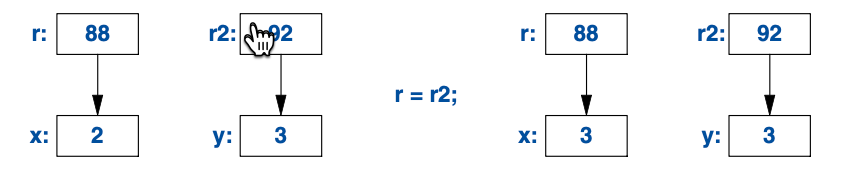
\includegraphics[width=.6\textwidth]{../images/ATourOfC++/1.png}
\label{}
\end{figure}
\section{User-Defined Types}
\label{sec:orgb04b042}
\subsection{Introduction}
\label{sec:org2e6cd40}
Types built out of other types using C++’s abstraction mechanisms are called \textbf{user-defined types}.
They are referred to as \textbf{classes} and \textbf{enumerations}.
\subsection{Structures}
\label{sec:orgf6f67de}
The \texttt{new} operator allocates memory from an area called the \textbf{free store} (also known as \textbf{dynamic
memory} and \textbf{heap}). Objects allocated on the free store are independent of the scope from which
they are created and ``live'' until they are destroyed using the \texttt{delete} operator
\subsection{Classes}
\label{sec:org4e2fcea}
The language mechanism for that is called a \textbf{class}. A class has a set of \textbf{members}, which can be
data, function, or type members. The interface is defined by the \texttt{public} members of a class, and
\texttt{private} members are accessible only through that interface.
\begin{minted}[]{c++}
class Vector {
    public:
        Vector(int s) :elem{new double[s]}, sz{s} { }
        double& operator[](int i) { return elem[i]; }
        int size() { return sz; }
    private:
        double* elem; // pointer to the elements
        int sz; // the number of elements
};
\end{minted}

\texttt{Vector(int)} defines how objects of type \texttt{Vector} are constructed. The constructor initializes the
\texttt{Vector} members using a member initializer list:
\begin{minted}[]{c++}
:elem{new double[s]}, sz{s}
\end{minted}
That is, we first initialize \texttt{elem} with a pointer to \texttt{s} elements of type \texttt{double} obtained from the
free store. Then, we initialize \texttt{sz} to \texttt{s}

Access to elements is provided by a subscript function, called \texttt{operator[]}. It returns a
reference to the appropriate element (a \texttt{double\&} allowing both reading and writing)

There is no \uline{fundamental} difference between a \texttt{struct} and a \texttt{class}; a \texttt{struct} is simply a class with
members \texttt{public} by default.
\subsection{Unions}
\label{sec:org95aef5e}
A \texttt{union} is a \texttt{struct} in which all members are allocated at the same address so that the \texttt{union}
occupies only as much space as its largest member. Naturally, a \texttt{union} can hold a value for
only one member at a time.
\begin{minted}[]{c++}
union Value {
    Node* p;
    int i;
};
\end{minted}
The language doesn’t keep track of which kind of value is held by a union, so the programmer
must do that:
\begin{minted}[]{c++}
enum Type { ptr, num }; // a Type can hold values ptr and num

struct Entry {
    string name;
    Type t;
    Value v; // use v.p if t==ptr; use v.i if t==num
};

void f(Entry* pe) {
    if (pe->t == num)
        cout << pe->v.i;
    // ...
}
\end{minted}
Maintaining the correspondence between a \textbf{type field} (here, \texttt{t}) and the type held in a \texttt{union} is
error-prone.

The standard library type, \texttt{variant}, can be used to eliminate most direct uses of unions. A
\texttt{variant} stores a value of one of a set of alternative types.
\begin{minted}[]{c++}
struct Entry {
    string name;
    variant<Node∗,int> v;
};

void f(Entry∗ pe) {
if (holds_alternative<int>(pe−>v))
    // does *pe hold an int?
    cout << get<int>(pe−>v);
    // get the int
    // ...
} 
\end{minted}

For many uses, a \texttt{variant} is simpler and safer to use than a \texttt{union}
\subsection{Enumerations}
\label{sec:org28a160e}
\begin{minted}[]{c++}
enum class Color { red, blue, green };
enum class Traffic_light { green, yellow, red };
Color col = Color::red;
Traffic_light light = Traffic_light::red;
\end{minted}

Note that enumerators (e.g., \texttt{red}) are in the scope of their \texttt{enum class}, so that they can be used
repeatedly in different \texttt{enum classes} without confusion. For example, \texttt{Color::red} is \texttt{Color} ’s \texttt{red}
which is different from \texttt{Traffic\_light::red}.

Enumerations are used to represent small sets of integer values. They are used to make code more
readable and less error-prone than it would have been had the symbolic (and mnemonic) enumerator
names not  been used.

The \texttt{class} after the \texttt{enum} specifies that an enumeration is strongly typed and that its
enumerators are scoped.
\begin{minted}[]{c++}
Color x = red; // error : which red?
Color y = Traffic_light::red;
// error: that red is not a Color
Color z = Color::red; // OK
\end{minted}

Similarly, we cannot implicitly mix \texttt{Color} and integer values:
\begin{minted}[]{c++}
int i = Color::red; // error: Color::red is not an int
Color c = 2; // initialization error: 2 is not a Color
\end{minted}

By default, an \texttt{enum class} has only assignment, initialization, and comparisons. However, an
enumeration is a user-defined type, so we can define operators for it:
\begin{minted}[]{c++}
Traffic_light& operator++(Traffic_light& t)
{ // prefix increment: ++ 
        switch (t) {
            case Traffic_light::green:
                return t=Traffic_light::yellow;
            case Traffic_light::yellow:
                return t=Traffic_light::red;
            case Traffic_light::red:
                return t=Traffic_light::green;
}
}
Traffic_light next = ++light;
// next becomes Traffic_light::green
\end{minted}

If you don’t want to explicitly qualify enumerator names and want enumerator values to be ints
(without the need for an explicit conversion), you can remove the \texttt{class} from \texttt{enum class} to get a
``plain'' \texttt{enum}. The enumerators from a ``plain'' \texttt{enum} are entered into the same scope as the
name of their enum and implicitly converts to their integer value

\begin{minted}[]{c++}
enum Color { red, green, blue };
int col = green;
\end{minted}
Here \texttt{col} gets the value 1. By default, the integer values of enumerators start with \texttt{0} and
increase by one for each additional enumerator.
\section{Modularity}
\label{sec:org48c80b6}
\subsection{Introduction}
\label{sec:org20845ac}
A \textbf{declaration} specifies all that’s needed to use a function or a type. For example:
\begin{minted}[]{c++}
double sqrt(double);
// the square root function takes a double and returns a double
class Vector {
    public:
        Vector(int s);
        double& operator[](int i); int size();
    private:
        double∗ elem; // elem points to an array of
                      // sz doubles int sz;
};        
\end{minted}

The key point here is that the function bodies, the function \textbf{definitions}, are ``elsewhere''

The definition of \texttt{sqrt()} will look like this:
\begin{minted}[]{c++}
double sqrt(double d) // definition of sqrt()
{
    // ... algorithm as found in math textbook ...
}
\end{minted}

For \texttt{vector}, we need to define
\begin{minted}[]{c++}
Vector::Vector(int s) // definition of the constructor
    :elem{new double[s]}, sz{s}
     // initialize members
{
}
double& Vector::operator[](int i) {
    // definition of subscripting
    return elem[i];
}
int Vector::size() {
    // definition of size()
    return sz;
}
\end{minted}
\subsection{Separate Compilation}
\label{sec:orgc0dd8eb}
C++ supports a notion of separate compilation where user code sees only declarations of the
types and functions used. The definitions of those types and functions are in separate source
files and are compiled separately.

This can be used to organize a program into a set of semi-independent code fragments. Such
separation can be used to minimize compilation times and to strictly enforce sepa- ration of
logically distinct parts of a program (thus minimizing the chance of errors). A library is often
a collection of separately compiled code fragments (e.g., functions).

Typically, we place the declarations that specify the interface to a module in a file with a
name indicating its intended use. Example:
\begin{minted}[]{c++}
// Vector.h:
class Vector {
    public:
        Vector(int s);
        double& operator[](int i); int size();
    private:
        double∗ elem;
        int sz;
};
\end{minted}

This declaration would be placed in a file \texttt{Vector.h}. Users then \textbf{include} that file, called a
\textbf{header file}, to access that interface. For example:
\begin{minted}[]{c++}
// user.cpp:
#include "Vector.h" // get Vector’s interface
#include <cmath> // get the standard-library
                 // math function interface including sqrt()
double sqrt_sum(Vector& v)
{
    double sum = 0;
    for (int i=0; i!=v.size(); ++i)
        sum+=std::sqrt(v[i]);
    return sum;
}
\end{minted}

To help the compiler ensure consistency, the \texttt{.cpp} file providing the implementation of \texttt{Vector}
will also include the .h file providing its interface:
\begin{minted}[]{c++}
// Vector.cpp:
#include "Vector.h" // get Vector’s interface
                
Vector::Vector(int s)
    :elem{new double[s]}, sz{s}
{    
}
double& Vector::operator[](int i)
{
    return elem[i];
}
int Vector::size()
{
    return sz;
}
\end{minted}

The code in \texttt{user.cpp} and \texttt{Vector.cpp} shares the \texttt{Vector} interface information presented in
\texttt{Vector.h}, but the two files are otherwise independent and can be separately compiled.

A \texttt{.cpp} file that is compiled by itself (including the h files it \texttt{\#includes}) is called a
\textbf{translation unit}. A program can consist of many thousand translation units.
\subsection{Modules (C++20)}
\label{sec:org69d74b0}
The use of \texttt{\#includes} is a very old, error-prone, and rather expensive way of composing programs
out of parts. If you \texttt{\#include header.h} in 101 translation units, the text of \texttt{header.h} will be
processed by the compiler 101 times. If you \texttt{\#include header1.h} before \texttt{header2.h} the declarations
and macros in \texttt{header1.h} might affect the meaning of the code in \texttt{header2.h}. If instead you
\texttt{\#include header2.h} before \texttt{header1.h}, it is \texttt{header2.h} that might affect the code in \texttt{header1.h}.
Obviously, this is not ideal, and in fact it has been a major source of cost and bugs since 1972
when this mechanism was first introduced into C.

Consider how to express the \texttt{Vector} and \texttt{sqrt\_sum()} example from §3.2 using \texttt{modules}:
\begin{minted}[]{c++}
// file Vector.cpp:
module; // this compilation will define a module
// ... here we put stuff that Vector might
// need for its implementation ...
export module Vector; // defining the module called "Vector"

export class Vector {
    public:
        Vector(int s);
        double& operator[](int i); int size();
    private:
        double∗ elem; // elem points to an array of sz doubles
        int sz;
};

Vector::Vector(int s)
:elem{new double[s]}, sz{s}
{
}

double& Vector::operator[](int i)
{
return elem[i];
}

int Vector::size()
{
return sz;
}

export int size(const Vector& v) { return v.size(); }
\end{minted}
This defines a module called \texttt{Vector}, which exports the class Vector, all its member functions,
and the non-member function \texttt{size()}

The way we use this module is to \texttt{import} it where we need it. For example:.
\begin{minted}[]{c++}
// file user.cpp:
// 
import Vector; // get Vector’s interface
#include <cmath>

double sqrt_sum(Vector& v)
{
    double sum = 0;
    for (int i=0; i!=v.size(); ++i)
        sum+=std::sqrt(v[i]);
    return sum;
}
\end{minted}

The differences between headers and modules are not just syntactic.
• A module is compiled once only (rather than in each translation unit in which it is used).
• Two modules can be \texttt{imported} in either order without changing their meaning.
• If you import something into a module, users of your module do not implicitly gain access
   to (and are not bothered by) what you imported: \texttt{import} is not transitive.
\subsection{Namespaces}
\label{sec:org3bdd209}
C++ offers \textbf{namespaces} as a mechanism for expressing that some declarations belong together and
that their names shouldn’t clash with other names

\begin{minted}[]{c++}
namespace My_code {
    class complex {
        // ...
    };
    complex sqrt(complex);
    // ...
    int main();
}

int My_code::main()
{
    complex z {1,2};
    auto z2 = sqrt(z);
    std::cout << '{' << z2.real() << ',' << z2.imag() << "}\n";
    // ...
}

int main()
{
    return My_code::main();
}
\end{minted}
By putting my code into the namespace \texttt{My\_code}, I make sure that my names do not conflict
with the standard-library names in namespace \texttt{std}

If repeatedly qualifying a name becomes tedious or distracting, we can bring the name into a
scope with a \texttt{using}-declaration:
\begin{minted}[]{c++}
void my_code(vector<int>& x, vector<int>& y)
{
    using std::swap; // ...
    swap(x,y);
    other::swap(x,y); // ...
}
\end{minted}

To gain access to all names in the standard-library namespace, we can use a \texttt{using}-directive:
\begin{minted}[]{c++}
using namespace std;
\end{minted}
\subsection{Error Handling}
\label{sec:org5e7dcd5}
\subsubsection{Exceptions}
\label{sec:orgf33e053}
Consider again the \texttt{Vector} example.

Assuming that out-of-range access is a kind of error that we want to recover from, the solution
is for the \texttt{Vector} implementer to detect the attempted out-of-range access and tell the user
about it. The user can then take appropriate action. For example, \texttt{Vector::operator[]()} can
detect an attempted out-of-range access and throw an \texttt{out\_of\_range} exception:
\begin{minted}[]{c++}
double& Vector::operator[](int i)
{
    if (i<0 || size()<=i)
        throw out_of_range{"Vector::operator[]"};
    return elem[i];
}
\end{minted}
The \texttt{throw} transfers control to a handler for exceptions of type \texttt{out\_of\_range} in some function that
directly or indirectly called \texttt{Vector::operator[]()}. To do that, the implementation will \textbf{unwind}
the function call stack as needed to get back the context of that caller. That is, the exception
handling mechanism will exit scopes and functions as needed to get back to a caller that has
expressed interest in handling that kind of exception, invoking destructors (§4.2.2) along the
way as needed. For example:

\begin{minted}[]{c++}
void f(Vector& v) {
// ...
    try { // exceptions here are handled by
          // the handler defined below
        v[v.size()] = 7; // try to access beyond the end of v
    }
    catch (out_of_range& err) {
    // ... handle range error ...
        cerr << err.what() << '\n';
    }
    // ...
}
\end{minted}

We put code for which we are interested in handling exceptions into a \texttt{try}-block. The attempted
assignment to \texttt{v[v.size()]} will fail. Therefore, the \texttt{catch}-clause providing a handler for
exceptions of type \texttt{out\_of\_range} will be entered. The \texttt{out\_of\_range} type is defined in the standard
library (in \texttt{<stdexcept>}) and is in fact used by some standard-library container access
functions.

The main technique for making error handling simple and systematic (called \textbf{Resource Acquisition
Is Initialization}; RAII) is explained in §4.2.2. The basic idea behind RAII is for a constructor
to acquire all resources necessary for a class to operate and have the destructor release all
resources, thus making resource release guaranteed and implicit.

A function that should never throw an exception can be declared \texttt{noexcept}. For example:
\begin{minted}[]{c++}
void user(int sz) noexcept {
    Vector v(sz);
    iota(&v[0],&v[sz],1); // fill v with 1,2,3,4...
    // ...
}
\end{minted}
\subsubsection{Invariants}
\label{sec:orgd403b22}
The use of exceptions to signal out-of-range access is an example of a function checking its
argument and refusing to act because a basic assumption, a \textbf{precondition}, didn’t hold
\begin{minted}[]{c++}
Vector::Vector(int s)
{
    if (s<0)
        throw length_error{"Vector constructor: negative size"};
    elem = new double[s];
    sz = s;
}
\end{minted}

If operator \texttt{new} can’t find memory to allocate, it throws a \texttt{std::bad\_alloc}.
\begin{minted}[]{c++}
void test()
{
    try {
        Vector v(−27);
    }
    catch (std::length_error& err) {
// handle negative size
    }
    catch (std::bad_alloc& err) {
// handle memory exhaustion
    }
}
\end{minted}

Often, a function has no way of completing its assigned task after an exception is thrown. Then,
‘‘handling’’ an exception means doing some minimal local cleanup and rethrowing the exception.
\begin{minted}[]{c++}
void test()
{
    try {
        Vector v(−27);
    }
    catch (std::length_error&) {
        // do something and rethrow
        cerr << "test failed: length error\n";
        throw; // rethrow
    }
    catch (std::bad_alloc&) {
        // Ouch! this program is not designed to handle memory exhaustion
        std::terminate(); // terminate the program
    }
}
\end{minted}
\subsubsection{Error-Handling Alternatives}
\label{sec:org870e77e}
Throwing an exception is not the only way of reporting an error that cannot be handled locally.
A function can indicate that it cannot perform its allotted task by:
• throwing an exception
• somehow return a value indicating failure
• terminating the program (by invoking a function like \texttt{terminate()}, \texttt{exit()}, or \texttt{abort())}.


One way to ensure termination is to add \texttt{noexcept} to a function so that a \texttt{throw} from anywhere in
the function’s implementation will turn into a \texttt{terminate()}.
\subsubsection{Contracts}
\label{sec:org5e4232e}
The standard library offers the debug macro, \texttt{assert()}, to assert that a condition must hold at
run time. For example:
\begin{minted}[]{c++}
void f(const char∗ p)
{
    assert(p!=nullptr);
    // p must not be the nullptr
}
\end{minted}
If the condition of an \texttt{assert()} fails in ``debug mode'', the program terminates
\subsubsection{Static Assertions}
\label{sec:org15c8779}
Exceptions report errors found at run time. If an error can be found at compile time, it is
usually preferable to do so.

The \texttt{static\_assert} mechanism can be used for anything that can be expressed in terms of constant
expressions
\begin{minted}[]{c++}
constexpr double C = 299792.458; // km/s
void f(double speed)
{
    constexpr double local_max = 160.0/(60∗60); // 160 km/h == 160.0/(60*60) km/s
    static_assert(speed<C,"can't go that fast"); // error: speed must be a constant
    static_assert(local_max<C,"can't go that fast"); // OK
    // ...
}
\end{minted}

In general, \texttt{static\_assert(A,S)} prints \texttt{S} as a compiler error message if \texttt{A} is not \texttt{true}. If you
don’t want a specific message printed, leave out the \texttt{S} and the compiler will supply a default message:

\section{Classes}
\label{sec:org161a312}
\subsection{Introduction}
\label{sec:org9e1bf6a}
\subsection{Concrete Types}
\label{sec:org5688d74}
The basic idea of \textbf{concrete classes} is that they behave ‘‘just like built-in types.’’
\subsubsection{An Arithmetic Type}
\label{sec:org1608917}
\begin{minted}[]{c++}
class complex {
    double re, im; // representation: two doubles
    public:
        // construct complex from two scalars
        complex(double r, double i) :re{r}, im{i} {}
        // construct complex from one scalar
        complex(double r) :re{r}, im{0} {}
        // default complex: {0,0}
        complex() :re{0}, im{0} {}
        
        double real() const { return re; }
        void real(double d) { re=d; }
        double imag() const { return im; }
        void imag(double d) { im=d; }
        
        complex& operator+=(complex z) {
            re+=z.re; // add to re and im im+=z.im;
            return *this; // and return the result
        }
        complex& operator-=(complex z) {
            re-=z.re;
            im-=z.im;
            return *this;
        }
        complex& operator*=(complex); // defined out-of-class somewhere
        complex& operator/=(complex); // defined out-of-class somewhere
};
\end{minted}

\texttt{complex} must be efficient or it will remain unused. This implies that simple operations must be
inlined. That is, simple operations (such as constructors, \texttt{+=}, and \texttt{imag()}) must be implemented
without function calls in the generated machine code. \textbf{Functions defined in a class are inlined
by default}. It is possible to explicitly request inlining by preceding a function declaration
with the keyword \texttt{inline}

A constructor that can be invoked without an argument is called a \textbf{default constructor}.

The \texttt{const} specifiers on the functions returning the real and imaginary parts indicate that these
functions do not modify the object for which they are called. A \texttt{const} member function can be
invoked for both \texttt{const} and non-\texttt{const} objects, but a non-\texttt{const} member function can only be
invoked for non-\texttt{const} objects. \href{https://stackoverflow.com/questions/3141087/what-is-meant-with-const-at-end-of-function-declaration}{stackexchange}

\begin{minted}[]{c++}
complex z = {1,0};
const complex cz {1,3};
z = cz; // OK: assigning to a non-const variable
cz = z; // error: complex::operator=() is a non-const member function double
x = z.real(); // OK: complex::real() is a const member function
\end{minted}

Many useful operations do not require direct access to the representation of complex, so they
can be defined separately from the class definition:
\begin{minted}[]{c++}
complex operator+(complex a, complex b) { return a+=b; }
complex operator−(complex a, complex b) { return a-=b; }
complex operator−(complex a) { return {−a.real(), −a.imag()}; }
complex operator∗(complex a, complex b) { return a*=b; }
complex operator/(complex a, complex b) { return a/=b; }
\end{minted}

The compiler converts operators involving complex numbers into appropriate function calls. For
example, \texttt{c!=b} means operator \texttt{!=(c,b)} and \texttt{1/a} means operator \texttt{/(complex\{1\},a)}.

User-defined operators (``overloaded operators'') should be used cautiously and conventionally.
The syntax is fixed by the language, so you can’t define a unary \texttt{/}. Also, it is not possible to
change the meaning of an operator for built-in types, so you can’t redefine \texttt{+} to subtract \texttt{ints}.
\subsubsection{A Container}
\label{sec:orgf2d0035}
A \textbf{container} is an object holding a collection of elements.

We need a mechanism to ensure that the memory allocated by the constructor is deallocated; that
mechanism is a \textbf{destructor}

\begin{minted}[]{c++}
class Vector { public:
        Vector(int s) :elem{new double[s]}, sz{s}
        // constructor: acquire resources
        {
            // initialize elements
            for (int i=0; i!=s; ++i)
                elem[i]=0;
        }
        // destructor: release resources
        ~Vector() { delete[] elem; }
        
        double& operator[](int i);
        int size() const;
        
    private:
        double* elem; // elem points to an array of sz doubles
        int sz;
};
\end{minted}

\texttt{Vector}'s constructor allocates some memory on the free store (also called the \textbf{heap} or \textbf{dynamic}
\textbf{store}) using the \texttt{new} operator. The destructor cleans up by freeing that memory using the
\texttt{delete[]} operator. Plain \texttt{delete} deletes an individual object, \texttt{delete[]} deletes an array.

The technique of acquiring resources in a constructor and releasing them in a destructor, known
as \textbf{Resource Acquisition Is Initialization} or \textbf{RAII}, allows us to eliminate ``naked \texttt{new}
operations'', that is, to avoid allocations in general code and keep them buried inside the
implementation of well-behaved abstractions.
\subsubsection{Initializing Containers}
\label{sec:orgf6fb40e}
\begin{itemize}
\item \textbf{Initializer-list constructor}: Initialize with a list of elements.
\item \texttt{push\_back()}: Add a new element at the end of (at the back of) the sequence.
\end{itemize}


\begin{minted}[]{c++}
class Vector {
    public:
        // initialize with a list of doubles
        Vector(std::initializer_list<double>); 
        // ...
        // add element at end, increasing the size by one 
        void push_back(double);
        // ...
};
\end{minted}

The \texttt{push\_back()} is useful for input of arbitrary numbers of elements
\begin{minted}[]{c++}
Vector read(istream& is) {
    Vector v;
    for (double d; is>>d; ) // read floating-point values into d
        v.push_back(d); // add d to v return v;
}
\end{minted}

The input loop is terminated by an end-of-file or a formatting error.

The way to provide Vector with a move constructor, so that returning a potentially huge amount
of data from read() is cheap
\begin{minted}[]{c++}
Vector v = read(cin); // no copy of Vector elements here
\end{minted}

The \texttt{std::initializer\_list} used to define the initializer-list constructor is a standard-library
type known to the compiler: when we use a \texttt{\{\}}-list, such as \texttt{\{1,2,3,4\}}, the compiler will create
an object of type \texttt{initializer\_list} to give to the program. So, we can write:
\begin{minted}[]{c++}
 // v1 has 5 elements Vector
Vector v1 = {1,2,3,4,5};
// v2 has 4 elements
v2 = {1.23, 3.45, 6.7, 8};
\end{minted}
\texttt{Vector}'s initializer-list constructor might be defined like this:
\begin{minted}[]{c++}
Vector::Vector(std::initializer_list<double> lst) // initialize with a list
    :elem{new double[lst.size()]}, sz{static_cast<int>(lst.size())}
{
    copy(lst.begin(),lst.end(),elem); // copy from lst into elem (§12.6)
}
\end{minted}

Unfortunately, the standard-library uses \texttt{unsigned} integers for sizes and subscripts, so I need
to use the ugly \texttt{static\_cast} to explicitly convert the size of the initializer list to an \texttt{int}

A \texttt{static\_cast} does not check the value it is converting; the programmer is trusted to use it
correctly.

Other casts are \texttt{reinterpret\_cast} for treating an object as simply a sequence of bytes and
\texttt{const\_cast} for ``casting away \texttt{const}.''
\subsection{Abstract Types}
\label{sec:orgf7a84fc}
an \textbf{abstract type} is a type that completely insulates a user from implementation details

First, we define the interface of a class \texttt{Container}, which we will design as a more abstract
version of our \texttt{Vector}:
\begin{minted}[]{c++}
class Container {
    public:
        // pure virtual function
        virtual double& operator[](int) = 0;
        // const member function (§4.2.1) 
        virtual int size() const = 0;
        // destructor (§4.2.2)
        virtual ~Container() {}
};
\end{minted}

The word \texttt{virtual} means ``may be redefined later in a class derived from this one'', and a function
declared \texttt{virtual} is called a \textbf{virtual function}.

A class derived from \texttt{Container} provides an implementation for the \texttt{Container} interface. The
curious \texttt{=0} syntax says the function is \textbf{pure virtual}; that is, some class derived from Container
must define the function. Thus, it is not possible to define an object that is just a Container.
For example:
\begin{minted}[]{c++}
Container c; // error: there can be no objects of an abstract class
Container∗ p = new Vector_container(10); // OK: Container is an interface
\end{minted}

A \texttt{Container} can only serve as the interface to a class that implements its \texttt{operator[]()} and
\texttt{size()} functions. A class with a pure virtual function is called an \textbf{abstract class}.

This \texttt{Container} can be used like this:
\begin{minted}[]{c++}
void use(Container& c) {
    const int sz = c.size();
    for (int i=0; i!=sz; ++i)
        cout << c[i] << '\n';
}
\end{minted}

Note how \texttt{use()} uses the \texttt{Container} interface in complete ignorance of implementation details. It
uses \texttt{size()} and \texttt{[]} without any idea of exactly which type provides their implementation. A
class that provides the interface to a variety of other classes is often called a \textbf{polymorphic
type}.

As is common for abstract classes, \texttt{Container} does not have a \uline{constructor}. After all, it does not
have any data to initialize. On the other hand, \texttt{Container} does have a destructor and that
destructor is \texttt{virtual}, so that classes derived from \texttt{Container} can provide implementations.
Again, that is common for abstract classes because they tend to be manipulated through
references or pointers, and someone destroying a \texttt{Container} through a pointer has no idea what
resources are owned by its implementation;

For \texttt{Container} to be useful, we have to implement a container that implements the functions
required by its interface. For that, we could use the concrete class \texttt{Vector}:
\begin{minted}[]{c++}
class Vector_container : public Container {
    // Vector_container implements Container
    public:
        Vector_container(int s) : v(s) { } // Vector of s elements
        ~Vector_container() {}
        
        double& operator[](int i) override { return v[i]; }
        int size() const override { return v.size(); }
    private:
        Vector v;
};
\end{minted}
The \texttt{:public} can be read as ``is derived from'' or ``is a subtype of.'' Class \texttt{Vector\_container} is
said to be \textbf{derived} from class \texttt{Container}, and class \texttt{Container} is said to be a \textbf{base} of class
\texttt{Vector\_container}. An alternative terminology calls \texttt{Vector\_container} and \texttt{Container} \textbf{subclass} and
\textbf{superclass}, respectively. The derived class is said to inherit members from its base class, so
the use of base and derived classes is commonly referred to as \textbf{inheritance}.

The members \texttt{operator[]()} and \texttt{size()} are said to \textbf{override} the corresponding members in the base
class \texttt{Container}. I used the explicit \texttt{override} to make clear what’s intended. The use of \texttt{override}
is \uline{optional}, but being explicit allows the compiler to catch mistakes, such as misspellings of
function names or slight differences between the type of a \texttt{virtual} function and its intended
overrider. The explicit use of \texttt{override} is particularly useful in larger class hiearchies where
it can otherwise be hard to know what is supposed to override what.

The destructor (\texttt{\textasciitilde{}Vector\_container()}) overrides the base class destructor (\texttt{\textasciitilde{}Container()}). Note
that the member destructor (\texttt{\textasciitilde{}Vector()}) is implicitly invoked by its class's destructor
(\texttt{\textasciitilde{}Vector\_container()}).

For a function like \texttt{use(Container\&)} to use a Container in complete ignorance of implementation
details, some other function will have to make an object on which it can operate. For example:
\begin{minted}[]{c++}
void g() {
    Vector_container vc(10); // ... fill vc ...
    use(vc);
}
\end{minted}

Since \texttt{use()} doesn’t know about \texttt{Vector\_container}​s but only knows the \texttt{Container} interface, it will
work just as well for a different implementation of a Container. For example:
\begin{minted}[]{c++}
class List_container : public Container {
        // List_container implements Container 
        public:
        List_container() { } // empty List 
        List_container(initializer_list<double> il) : ld{il} { }
        ~List_container() {}
        double& operator[](int i) override;
        int size() const override { return ld.size(); }
    private:
        std::list<double> ld; // (standard-library) list of doubles
};
double& List_container::operator[](int i) {
    for (auto& x : ld) {
        if (i==0)
            return x;
        −−i;
    }
    throw out_of_range{"List container"};
}
\end{minted}

A function can create a \texttt{List\_container} and have \texttt{use()} use it:
\begin{minted}[]{c++}
void h() {
    List_container lc = { 1, 2, 3, 4, 5, 6, 7, 8, 9 };
    use(lc);
}
\end{minted}

The point is that \texttt{use(Container\&)} has no idea if its argument is a \texttt{Vector\_container}, a
\texttt{List\_container}, or some other kind of container; it doesn’t need to know. It can use any kind of
\texttt{Container}. It knows only the interface defined by \texttt{Container}. Consequently, \texttt{use(Container\&)}
needn’t be recompiled if the implementation of \texttt{List\_container} changes or a brand-new class
derived from Container is used.
\subsection{Virtual Functions}
\label{sec:org63ee07c}
Consider again the use of \texttt{Container}:
\begin{minted}[]{c++}
void use(Container& c) {
    const int sz = c.size();
    for (int i=0; i!=sz; ++i) cout << c[i] << '\n';
}
\end{minted}
\end{document}
